\documentclass[slovene,11pt,a4paper]{article}
%\usepackage{fullpage}
\usepackage[margin=2cm]{geometry}

\usepackage[T1]{fontenc}



%dodatni paketki:
\usepackage{graphicx}
\usepackage{amsmath,amsfonts,amsthm} %matematicni paket
\usepackage{color} % omogoča barvno pisanje
\usepackage[utf8]
{inputenc}
\usepackage[slovene]{babel} % slovenski jezik/hyphenation
\usepackage{hyperref} %naredi vse povezave rečerenc, kazala,...
\numberwithin{equation}{section} % Number equations within sections (i.e. 1.1, 1.2, 2.1, 2.2 instead of 1, 2, 3, 4)
\numberwithin{figure}{section} % Number figures within sections (i.e. 1.1, 1.2, 2.1, 2.2 instead of 1, 2, 3, 4)
\numberwithin{table}{section} % Number tables within sections (i.e. 1.1, 1.2, 2.1, 2.2 instead of 1, 2, 3, 4)
\usepackage{eurosym} %za znak €

\usepackage{mathrsfs}
\usepackage{mathabx} % za kemisjke smeri in naslednje 3 vstrice
\catcode`_=12
\begingroup\lccode`~=`_\lowercase{\endgroup\let~\sb}
\mathcode`_="8000

\usepackage{placeins}
\usepackage[margin=2cm]{geometry}



\begin{document}
\begin{titlepage}

\newcommand{\HRule}{\rule{\linewidth}{0.5mm}} % Defines a new command for the horizontal lines, change thickness here

\center % Center everything on the page

%----------------------------------------------------------------------------------------
%	LOGO
%----------------------------------------------------------------------------------------

%\includegraphics{Logo}\\[1cm] % Include a department/university logo - this will require the graphicx package
 
%----------------------------------------------------------------------------------------


\includegraphics[width=2cm]{slike/aaa}\\[0.5cm]
 
%----------------------------------------------------------------------------------------
%	NASLOV DELA
%----------------------------------------------------------------------------------------
\textit{Univerza v Ljubljani}\\
\textit{Fakulteta za {\color{red}matematiko in fiziko}}\\[0.5cm]

\emph{Oddelek za fiziko}\\[0.5cm] % Oddelek za fiziko


%----------------------------------------------------------------------------------------
%	TITLE SECTION
%--------------------------------------------------------------------------------------
\HRule \\[0.4cm]
\huge {\bfseries 1. naloga: Numerično reševanje Schrodingerjeve enačbe -1.del}\\[0.4cm] % NASLOV SEMINARJA
\HRule \\[0.5cm] 

 \textsc{\large Poročilo pri predmetu višje računske metode}\\
 \textsc{\large 2016/2017}\\[1cm] % SEMINASKO DELO
 
%----------------------------------------------------------------------------------------
%	AUTHOR SECTION
%----------------------------------------------------------------------------------------



% If you don't want a supervisor, uncomment the two lines below and remove the section above
\Large \emph{Avtor:}\\
Klemen \textsc{Rahne}\\
28152028\\[2cm]
%----------------------------------------------------------------------------------------
%	DATUM
%----------------------------------------------------------------------------------------

{\large \today } \\[0.5cm] % Date, change the \today to a set date if you want to be precise

	

\end{titlepage}


%----------------------------------------------------------------------------------------
%	KAZALO
%----------------------------------------------------------------------------------------

%\tableofcontents

%----------------------------------------------------------------------------------------
%	ZAČETEK TEKSTA
%----------------------------------------------------------------------------------------
\section{naloga}
Primerjali bomo metode reševanja Schrodingerjeve enačbe za en delec. Uporabili bomo eksplecitno metodo (Eulerjevo) ter implicitno metodo. Od omenjenih metod je eulerjeva metoda slabša, saj je že po nekaj korakih valovna funkcija divergira-to se lepo vidi iz grafa \ref{slika1}. Pri vseh metodah sem za začetno iteracijo uporabil osnovno valovno funkcijo za harmosnki oscilator. Oglejmo si še kako vpliva širina obravnavanega obočja na vrednost valovne funkcije.





\begin{figure}[h]
\label{slika1}
\begin{center}
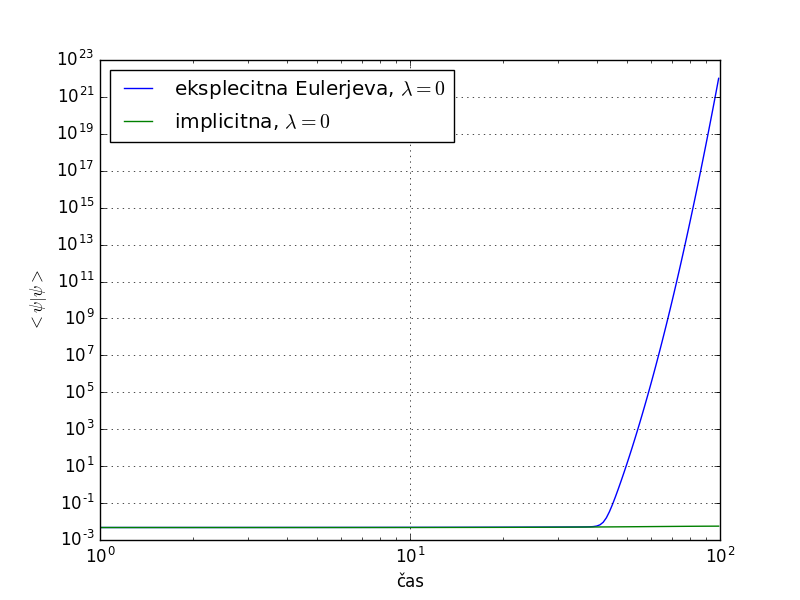
\includegraphics[scale=0.45]{slike/primerjava1.png}
\end{center}
\caption{Primerjava Eulerjeve metode in implicitne metode. V prostoru smo imeli dolžino $10$ in točke razdeljene na $0.1$, v času pa razmik $0.01$. Na zgornjem grafu je časovna enota v korakih (integer).}
\end{figure}


\begin{figure}[h]
\label{slika1}
\begin{center}
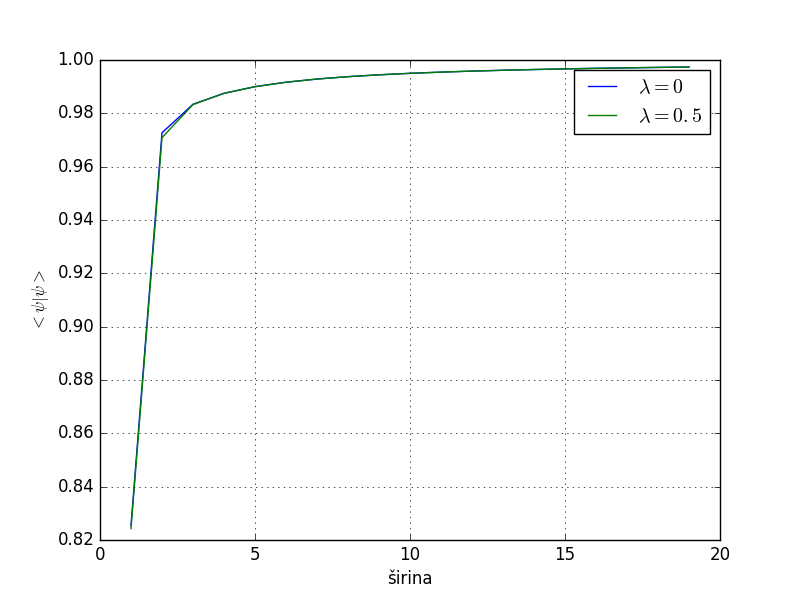
\includegraphics[scale=0.45]{slike/slika2.png}
\end{center}
\caption{Primerjava širine obravnavanega območja v enotah širine osnovne valovne funkcije. Ni presenetljivo, da z večanjem območja dobimo lepše rešitve. Dejansko obravnavano občje im dvojno širino, saj smo obravnavali območje $[-sirina,sirina]$. Za primerjavo smo vključili še dodaten anhramoski člen oblike $\lambda x^4$.}
\end{figure}


\newpage

\section{naloga}
Oglejmo si kako izgleda če osnosvno valovno funkcijo zamaknemo za razdaljo $a$. Pričakovati je, da se valovna funkcija šele po nekaj korakih stabilizirala okoli izhodišča potenciala.


\begin{figure}[!htb]
\centering
\begin{minipage}{0.5\textwidth}
\centering
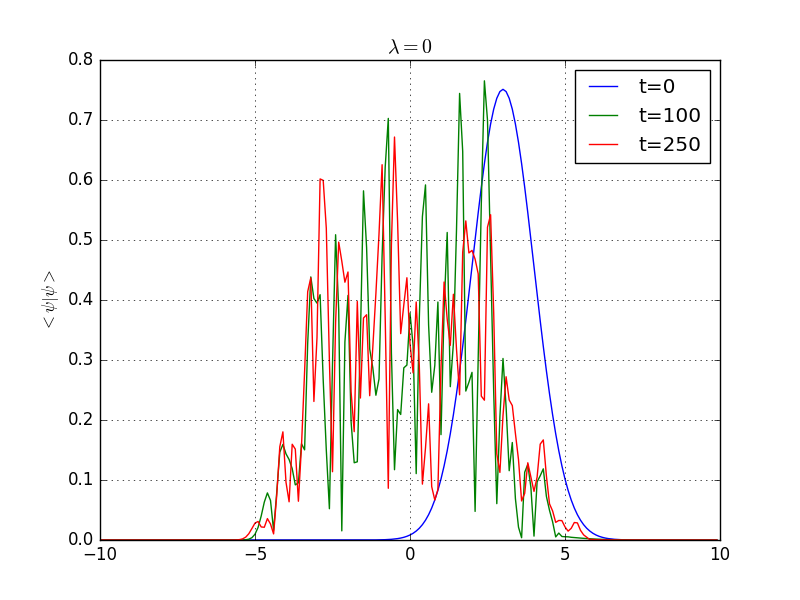
\includegraphics[scale=0.45]{slike/casovni_razvoj_izmika.png}
%\caption{first figure}
\end{minipage}\hfill
\begin{minipage}{0.5\textwidth}
\centering
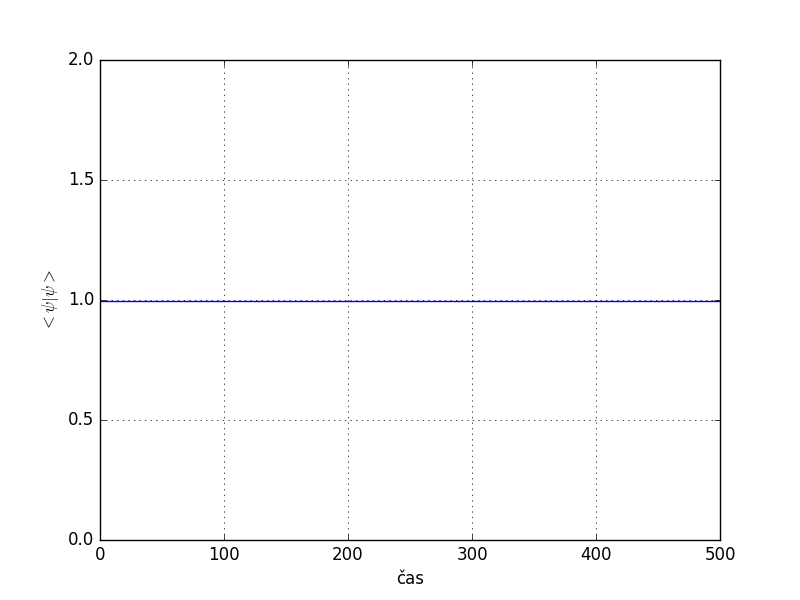
\includegraphics[scale=0.45]{slike/ohranjanje_delcev.png}
%\caption{second figure}
\end{minipage}

\caption{Na levem grafu vidimo časovni potek valovne funkcije po času. Na začetku je funkcija zelo jasno določena, kasneje se pa gaussova oblika "zamaže". Na desnem grafu vidimo, da se kljub zamazanosti gausove krivulje ohranja verjetnostna gostota.}
\end{figure}

\end{document}
